% Chapter Template

\chapter{Next Steps} % Main chapter title

\label{Chapter4} % Change X to a consecutive number; for referencing this chapter elsewhere, use \ref{ChapterX}

The progress has been on track so far, with regard to the semester 1 plan in the project proposal. The immediate next step is to further expand the flow filtering system, so that we can implement different  filters for different sensors (\ref{fig:flowfiltermul}). An preliminary graph of a complete flow filter is shown below, where each filter connects to one after the other to process frames with different sensors. 

\begin{figure}[!htbp]
	\caption{\label{fig:flowfiltermul}Flow Filter System with Multiple Filters}
	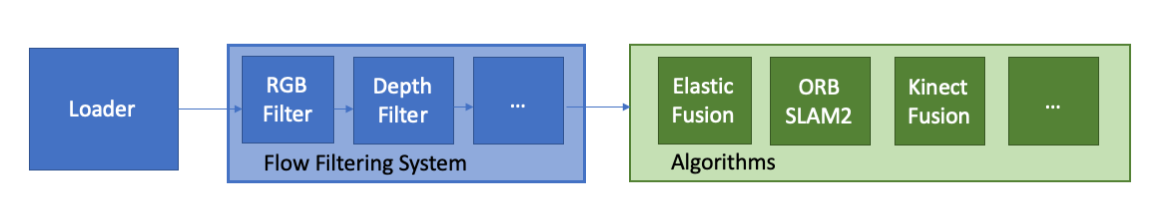
\includegraphics[width=14cm]{figures/flow-filter-complex.png}
	\centering
\end{figure}

Further next steps include organizing the flow filters into a module, and writing a documentation for the module. Ideally these tasks could be completed by the first half of semester 2, so that focus can be placed on experimenting the filtering system with different data sets and SLAM algorithms, as well as preparing capstone deliverable such as the thesis.